\definecolor{C1}{RGB}{226, 43, 41} % trx
\definecolor{C2}{RGB}{47, 96, 206} % tsl
\definecolor{C3}{RGB}{246, 175, 11} % chamfer

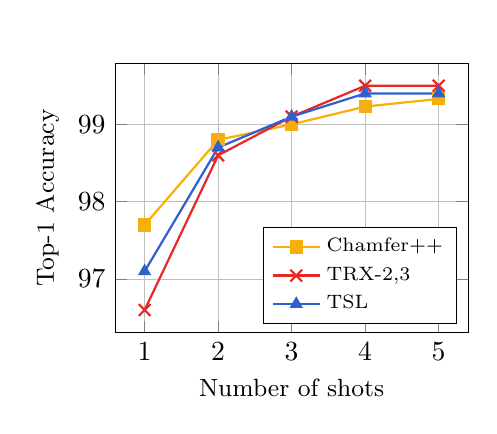
\begin{tikzpicture}
  \begin{axis}[
    width=0.5\linewidth,
    height=5cm, 
    xtick = {0,1,2,3,4,5},
  	legend cell align={left},
	legend pos=south east,
    legend style={font=\scriptsize}, 
    grid=both,
    xlabel={\small Number of shots},
    ylabel={\small Top-1 Accuracy},
    title={\ucf}
  ]
    \addplot [thick, color=C3, mark=square*,  mark size=2] coordinates {(1, 97.7) (2, 98.8) (3, 99) (4, 99.23) (5, 99.33)}; 
	\addlegendentry{Chamfer++}  
	
	\addplot [thick, color=C1,  mark=x,  mark size=3] coordinates {(1, 96.6) (2, 98.6) (3, 99.1) (4, 99.5) (5, 99.5)};   
	\addlegendentry{TRX-{2,3}}]
    
    \addplot [thick, color=C2, mark=triangle*,  mark size=2] coordinates {(1, 97.1)(2, 98.7) (3, 99.1) (4, 99.4) (5, 99.4)};  
	\addlegendentry{TSL}  
	
  \end{axis}
\end{tikzpicture}
